\documentclass[12pt, a4paper]{article}

\usepackage{ctex}
\usepackage{float, booktabs, parskip}
\usepackage{amsmath, amsthm, amssymb, mathrsfs, bm}
\usepackage{graphicx, subfigure, svg}
\usepackage{hyperref, endnotes}

\setlength{\parindent}{4em}
\setlength{\parskip}{1em}
\allowdisplaybreaks[4]




\title{{\Huge{\textbf{Report on Homework 2 \\}}} —— Deep Learning}
\author{刘滨瑞 \\ 2021012579 \quad 未央-水木12}

\begin{document}

\maketitle

\section{Language modeling with RNN}

    运行环境为：Windows 10 22H2，Python 3.9.18，PyTorch 1.12.1。

    \subsection{RNN for Language Modeling}

        使用Pytorch提供的nn.GRU类，我实现了基于GRU结构的循环神经网络，源代码参见./rnn/model.py的49-97行。

        我补全了train()函数和evaluate()函数，同时完善了模型训练与测试的基本框架，具体实现可以参见./rnn/main.py中使用注释框出的代码内容。

        取训练时的批大小为20，验证时的批大小为10；
        取最大序列长度为35；RNN堆叠层数为2；词嵌入维度数和隐藏层维度数均为256；
        使用Adam优化器，学习率固定为0.001；
        固定随机数种子为42；调用train()函数和evaluate()函数，共训练40个epoch，平均训练速度为2.5min per epoch。

        关于模型的训练与验证结果，我们将在下一节中同LSTM的实验结果一并展示、分析。

    \subsection{LSTM Implementation}

        参考原论文和课件中的相关公式，我还原了LSTM中的四个控制门，源代码参见./rnn/model.py中的Memory类。 \endnote{Hochreiter, S., and Schmidhuber, J. (1997). Long short-term memory. Neural computation.}
        在此基础上，我仿造nn.GRU的接口格式，完成了LSTM的整体结构，源代码参见./rnn/model.py中的MyLSTM类。

        保持上一节中所使用的超参数不变，调用train()函数和evaluate()函数，训练40个epoch，平均训练速度为4.5min per epoch。
        注意到在相同的超参数下，LSTM的训练效率明显低于GRU。

        训练过程中，GRU与LSTM在测试集、验证集上loss与perplexity的变化情况如图1、图2所示。

        \begin{figure}[htbp]
        \centering
        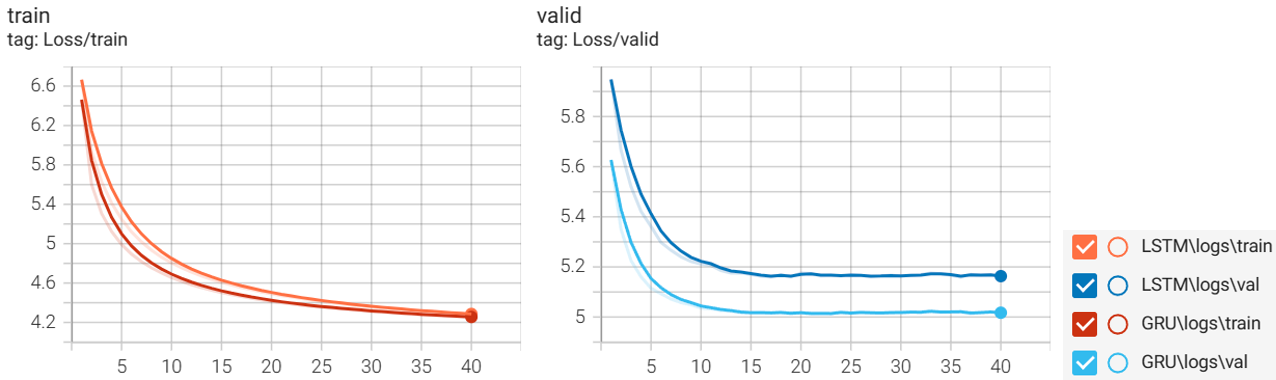
\includegraphics[width=1\textwidth]{./assets/rnn_loss.png}
        \caption{训练过程中GRU与LSTM的loss变化情况}
        \end{figure}

        \begin{figure}[htbp]
        \centering
        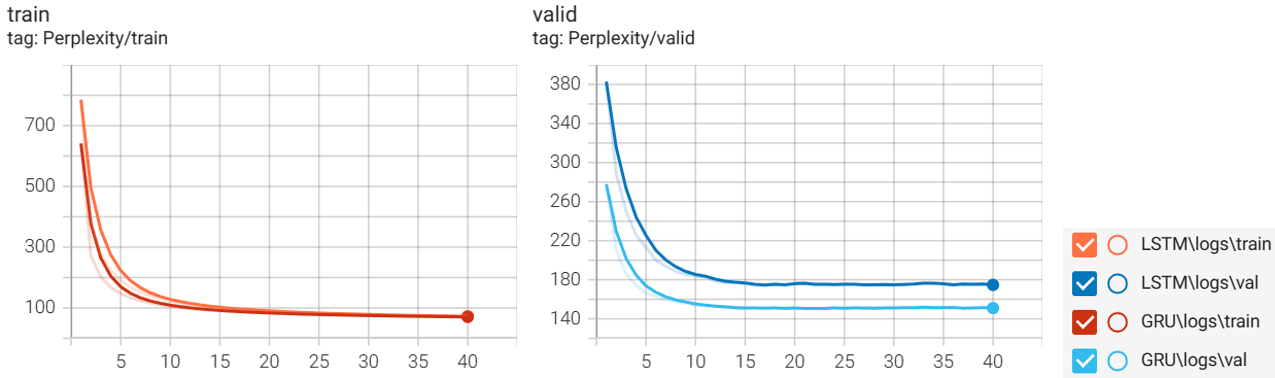
\includegraphics[width=1\textwidth]{./assets/rnn_perplexity.png}
        \caption{训练过程中GRU与LSTM的perplexity变化情况}
        \end{figure}

        可以看出，GRU和LSTM的收敛情况良好，在训练集上的loss最终均降低至4.25，perplexity最终均降低至70，其中GRU的收敛速度略快。
        而在验证集上，LSTM的loss最终降至5.16，perplexity最终降至175，而GRU的loss最终可降至5.02，perplexity最终可降至150。
        综上，可以认为GRU较LSTM更容易训练，具有更高的收敛速度，GRU的泛化能力也要略强于LSTM。

        在训练过程中，我们计算GRU与LSTM在测试集、验证集上的Top-1准确率和Top-5准确率，结果如图3、图4所示。

        \begin{figure}[htbp]
        \centering
        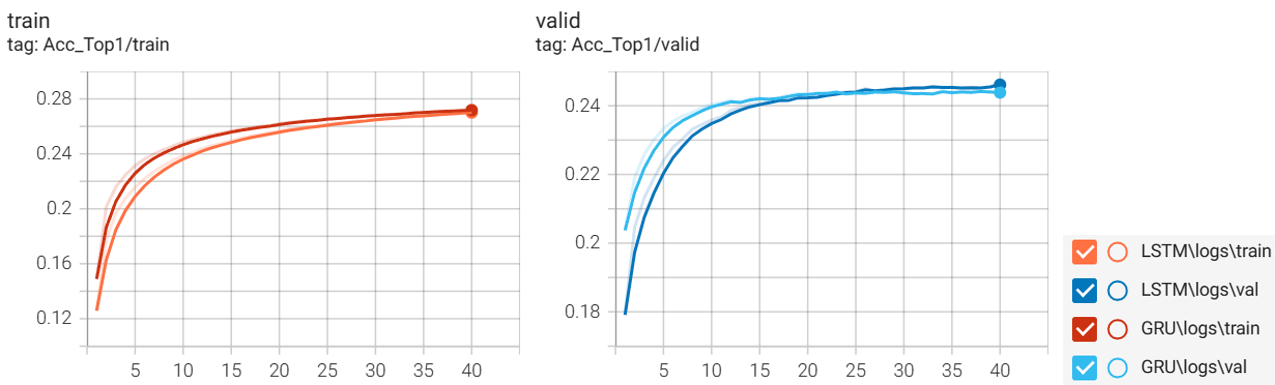
\includegraphics[width=1\textwidth]{./assets/rnn_acc_top1.png}
        \caption{训练过程中GRU与LSTM的Top-1准确率变化情况}
        \end{figure}

        \begin{figure}[htbp]
        \centering
        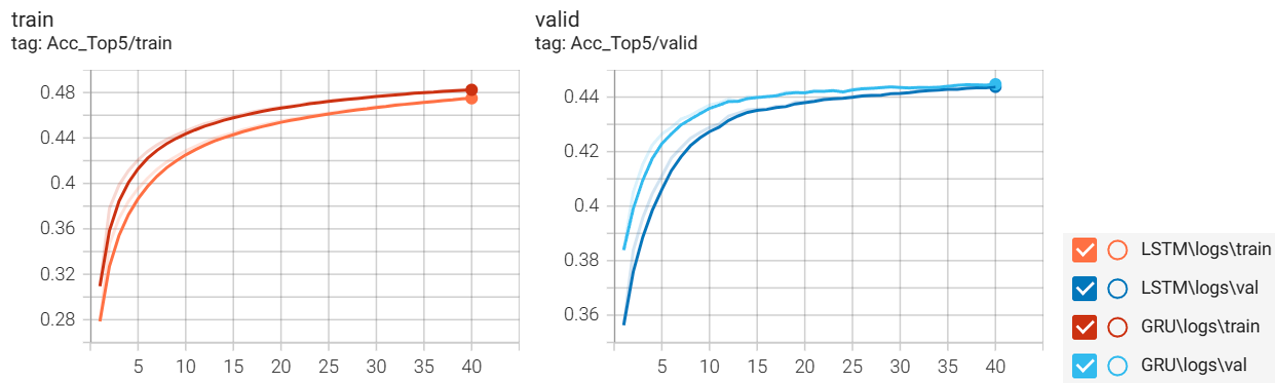
\includegraphics[width=1\textwidth]{./assets/rnn_acc_top5.png}
        \caption{训练过程中GRU与LSTM的Top-5准确率变化情况}
        \end{figure}

        可以看出，GRU和LSTM的准确率表现几乎一致，我们统计其最佳准确率，展示在表1中。

        结果显示，在训练集和测试集上，GRU和LSTM的Top-1准确率、Top-5准确率各有高低，但都没有明显的差距。
        因此，我们倾向与认为GRU与LSTM在语言学习任务中的性能是等同的。
        这证明了相对于LSTM，GRU所采用的简化结构的合理性与有效性。

        \begin{table}[htbp]
        \caption{GRU和LSTM的最佳准确率结果}
        \centering
        \begin{tabular}{ccc}
            \toprule
            model             & Top-1 Accuracy & Top-5 Accuracy \\
            \midrule
            GRU (train)       &     27.20\%    &     48.27\%    \\
            LSTM (train)      &     27.04\%    &     47.53\%    \\
            \midrule
            GRU (validation)  &     24.37\%    &     44.49\%    \\
            LSTM (validation) &     24.66\%    &     44.39\%
        \end{tabular}
        \end{table}

    \subsection{Inference using RNN}

        我补全了predict()函数，源代码参见./rnn/main.py。

        predict()函数使用了Beam Search和Auto-Regressive进行语言推理。
        其实现过程可分为如下若干步：

        \begin{enumerate}

        \item 首先，我们需要载入完成训练的RNN，这里使用的是GRU。然后，我们载入data\_loader提供的词表和词典，用于翻译。

        \item 我们先将待补全的句子token化，然后将其输入RNN中。
        RNN会输出一个Tensor，该Tensor的第一维代表着sequence。
        取该维度上的最后一位上的Tensor切片，即为模型给出的下一个词语的概率分布的预测。

        \item 基于此预测，我们即可以判断哪些词更有可能被填入句子的下一个位置。
        而在Beam Search中，我们总是保留前$K$个最有可能的词语选项。

        \item 对于$K$个词语中的每一个，我们都将其填入句子的末尾，视为已知，然后重新将整个句子输入RNN。
        重复Beam Search步骤，我们将得到$K^2$个最有可能的词语选项组合，我们仅保留其中$K$个联合概率最大的。

        \item 重复第4步，直到词语序列达到指定长度。

        \end{enumerate}

        值得一提的是，推理过程中的预测比例可以通过修改输入文本长度与指定序列长度的值调整。
        另外，Beam Search的搜索宽度$K$也是一个重要的参数，直接影响着推理的复杂度与效果。

        使用predict()函数，我们输入部分自定义文本和验证集中的文本，检查RNN的自回归推理结果。
        这部分的代码参见./rnn/inference.py文件。

        首先是部分自定义文本的输入。
        取$K = 10$，我们输入了以下三句文本，要求补充8个词语，结果如图5所示：

        \begin{enumerate}

        \item I am a student . I love

        \item I am a student . I live in America . I love

        \item I am a student . I live in America . I do not love money . I love

        \end{enumerate}

        \begin{figure}[htbp]
        \centering
        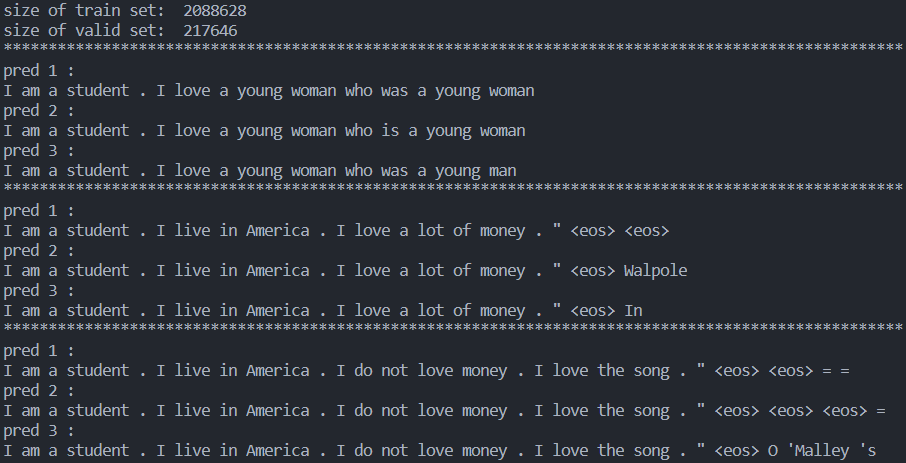
\includegraphics[width=1\textwidth]{./assets/rnn_predict.png}
        \caption{自定义文本的自回归推理结果}
        \end{figure}

        可以看出，模型能够理解输入语句的含义，并给出符合英文语法和简单逻辑的补全。

        然后，我们从验证集摘取10段语句，这10段语句的原文与摘取位置详见./rnn/inference.py文件。
        去掉这10段语句尾部的若干个词语，将它们输入模型，令其进行推理预测，结果如图6所示。

        \begin{figure}[htbp]
        \centering
        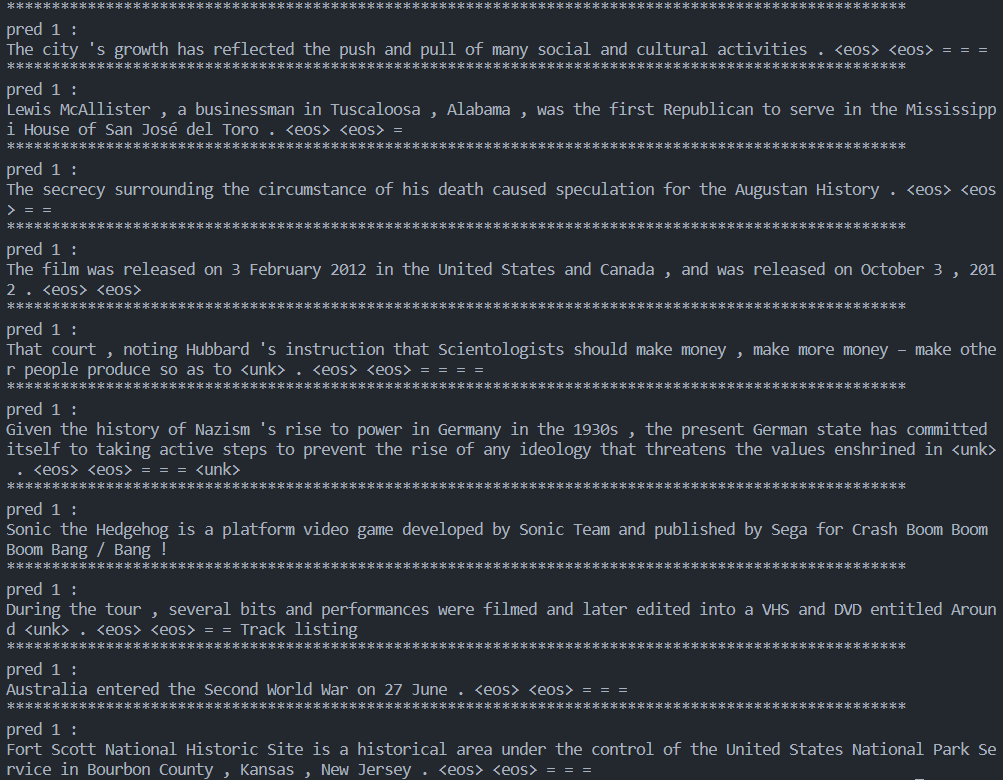
\includegraphics[width=1\textwidth]{./assets/rnn_valid.png}
        \caption{部分验证集文本的自回归推理结果}
        \end{figure}

        可以看出，预测结果有好有坏。
        第一句、第九句和第十句的补全效果较好，大致符合语法和逻辑，内容也与原文相近。
        而第二句、第五句和第八句的补全效果较差，有点不知所云。

        我认为，模型补全部分语句的效果较差，
        一方面是因为训练集规模过小，有一些知识性的内容——如Sonic是哪家公司制作的——不能够学习到；
        另一方面则是因为RNN对于自然语言特征的提取能力仍然有限，尚且不能够理解一些复杂的语法与逻辑。

    \subsection{Question Answering}

        使用字母级别的RNN的优势：

        我们注意到，在字母级别，RNN需要处理的仅仅是包含几十个字符的字母表，而非规模以万计的词汇表，
        这使得RNN中输入层和输出层的维度数可以大幅减小。
        另外，字母作词嵌入后的大小远小于单词作词嵌入后的大小。
        这都将使得模型的参数量和复杂度显著降低，同时也将允许模型能够处理更大的词汇量规模的任务。

        使用字母级别的RNN的劣势：

        在字母级别，RNN需要从字母层面理解自然语言，这一任务的难度非常高，
        这要求RNN在学习如何组织单词之前，还需要先学会如何拼写单词、理解单词。
        这一方面使得RNN需要更大规模的数据进行训练，提高了训练难度，
        另一方面也减小了RNN输出可被人类理解的文本的可能。

\section{Graph Neural Networks and Node2Vec}

    运行环境为：Windows 10 22H2，Python 3.9.18，PyTorch 1.12.1，Torch Geometric 2.0.3。

    \subsection{Task A and Task B}

        参考原论文，基于Pytorch Geometric库提供的MLP、GINConv等基本结构模块，我重新实现了GIN。 \endnote{Xu, K., Li, C., Tian, Y., Sonobe, T., Kawarabayashi, K., and Jegelka, S. (2018). How powerful are graph neural networks? In Proceedings of the International Conference on Learning Representations (ICLR).}
        为了让GIN具备更好的性能，我调整了dropout层和relu函数在网络中的位置，同时适当地调整了网络层数、隐藏层维度等超参数。
        源代码参见./gnn/gin.py。

        运行./gnn/gcn.py、./gnn/gat.py、./gnn/node2vec.py和./gnn/gin.py，
        记录模型在训练过程中的损失值变化情况，记录模型在训练集、验证集和测试集上的准确率变化情况，
        结果如图7，图8所示。

        \begin{figure}[htbp]
        \centering
        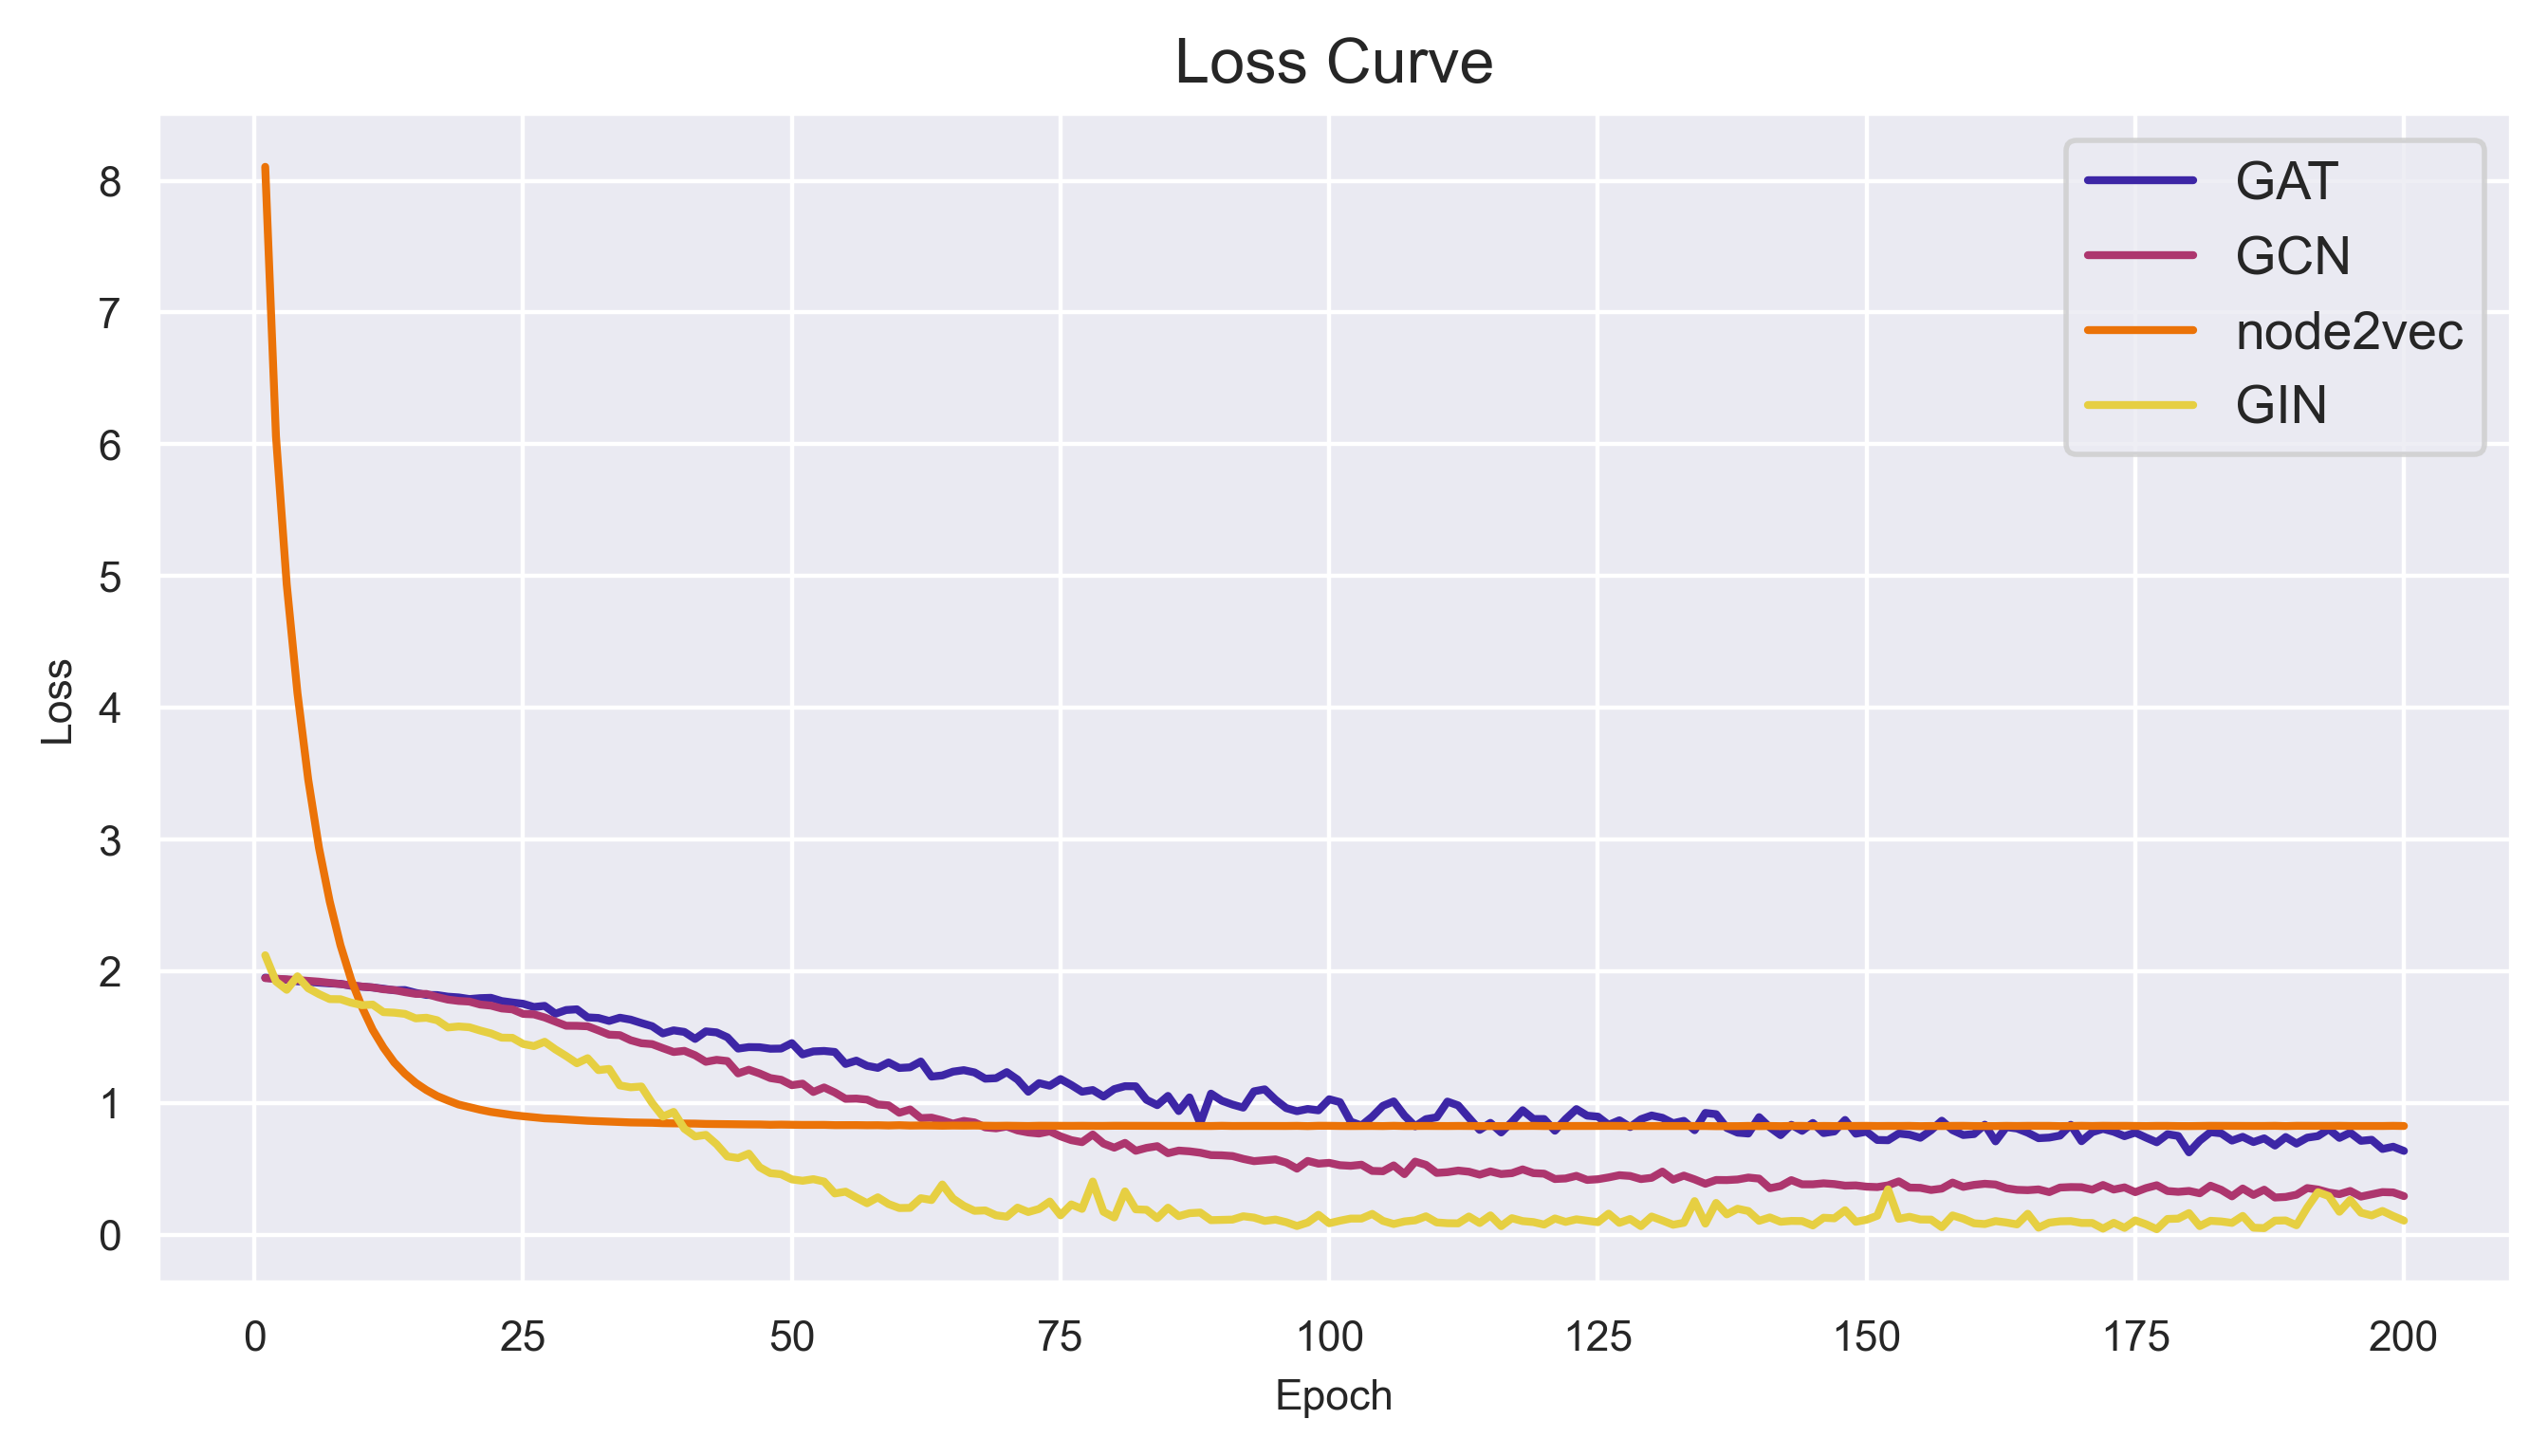
\includegraphics[width=1\textwidth]{./assets/gnn_loss.png}
        \caption{在训练过程中，各GNN的loss变化情况}
        \end{figure}

        可以看出，各模型的收敛情况良好。Node2Vec的收敛速度最快，GIN次之，GAT的收敛速度最慢。

        \begin{figure}[htbp]
        \centering
        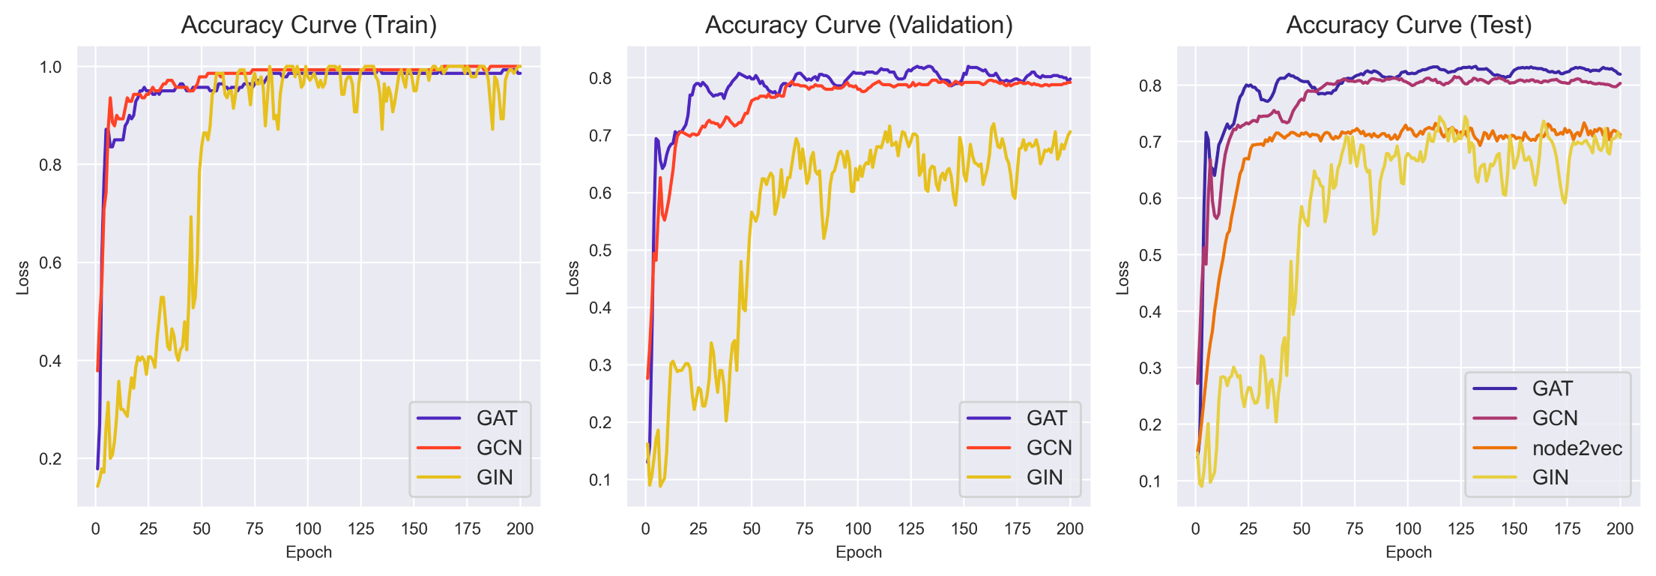
\includegraphics[width=1\textwidth]{./assets/gnn_acc.png}
        \caption{在训练过程中，各GNN的准确率变化情况}
        \end{figure}

        GAT、GAN和GIN都能够完全拟合训练集，最终在训练集上达到接近100\%的准确率。
        在验证集上，GAT、GAN的准确率可达80\%，GIN的准确率可达70\%。
        在测试集上，各模型的表现同验证集类似，GAT、GAN的最终准确率为80\%，Node2Vec、GIN的最终准确率为70\%。

        如图9所示，使用训练后的Node2Vec模型生成TSNE图。
        从图中可以直观地看出，Node2Vec对图数据集的分类效果良好。
        我们有理由相信，性能较Node2Vec更好的GAT、GAN等GNN模型同样可以较为成功地完成对图数据集的分类任务。

        \begin{figure}[htbp]
        \centering
        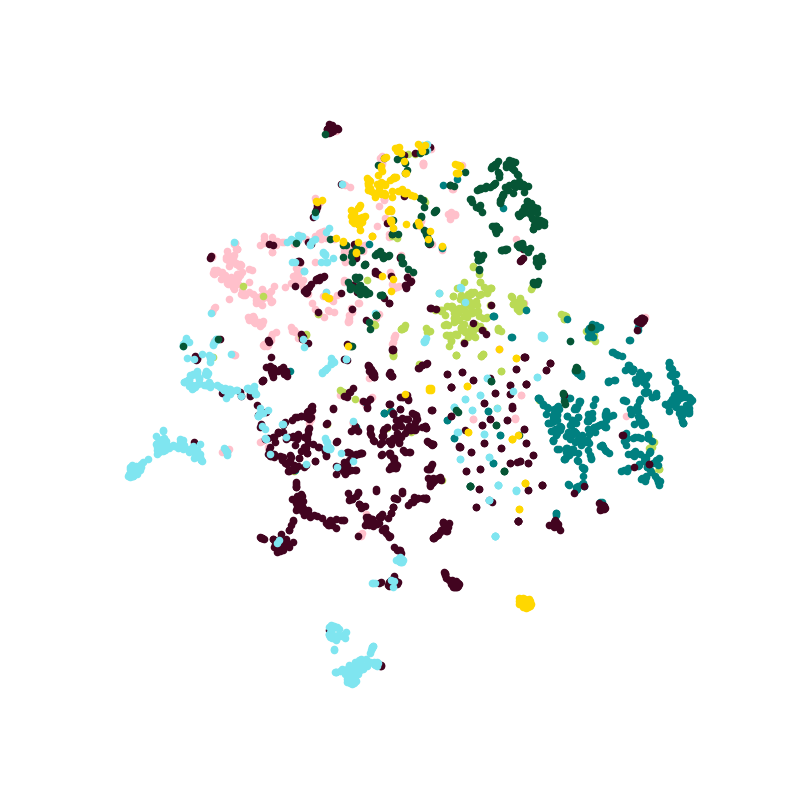
\includegraphics[width=1\textwidth]{./assets/visualization.png}
        \caption{Node2Vec模型生成的TSNE图}
        \end{figure}

\theendnotes

\end{document}
